\chapter{Theoretical Framework}
\label{ch:theoretical-framework}

Before starting with rehabilitate the main topic, some basic concepts, technical terms and underlying theory has to be explained.
This is important to faster read through the thesis without the need to interrupt the flow of thought.
In the following, a set of established theories and terms is explained which are not directly related to the thesis formulation, but essential to comprehend numerous contexts.

\section{Android UI}
\label{sec:android-ui}

To be able to use any of the things displayed on the mobile device, some concepts of \gls{ui} programming must be shown.
A \gls{ui} enables the user to view the applications data on the screen but also to interact with the device especially on mobile devices \cite{android_ui_layer}.

The main challenge is to bring the application data in the right format, so that the display can interpret the instructions to draw the elements.
Each mobile phone with the Android \gls{os} has a basic set of native functions through which the \gls{ui} can be drawn and updated, a so-called \gls{api}.
These functions can be very general to instruct drawing a whole component such as an alert box, or they can be very specific as drawing single rectangles in a canvas.

The rough transition from the application data (data layer) to the display data (ui layer) is depicted in figure \ref{fig:android_udf}.
The application data is transformed, concatenated or filtered to be saved in a view model, which represents the state for each view.
The view model is then layed out to multiple \gls{ui} elements.
E.g.\ they are loaded in the Android activity via view layouts~\cite{android_draw_views} or composed in a declarative approach~\cite{android_jetpack_compose}.
It is generally advised to use a \gls{udf}.
This ensures that the data is only changed in one place and doesn't get out of sync between \gls{ui} elements, the view model and the data layer.
The \gls{ui} can also register user inputs (like a button press) and report them back to the view model.
The view model then updates the application data, if needed, and then also reports the current \gls{ui} state back to the UI elements to be rerendered.

\begin{figure}[htbp!]
    \centering
    \begin{subfigure}[b]{0.5\textwidth}
        \centering
        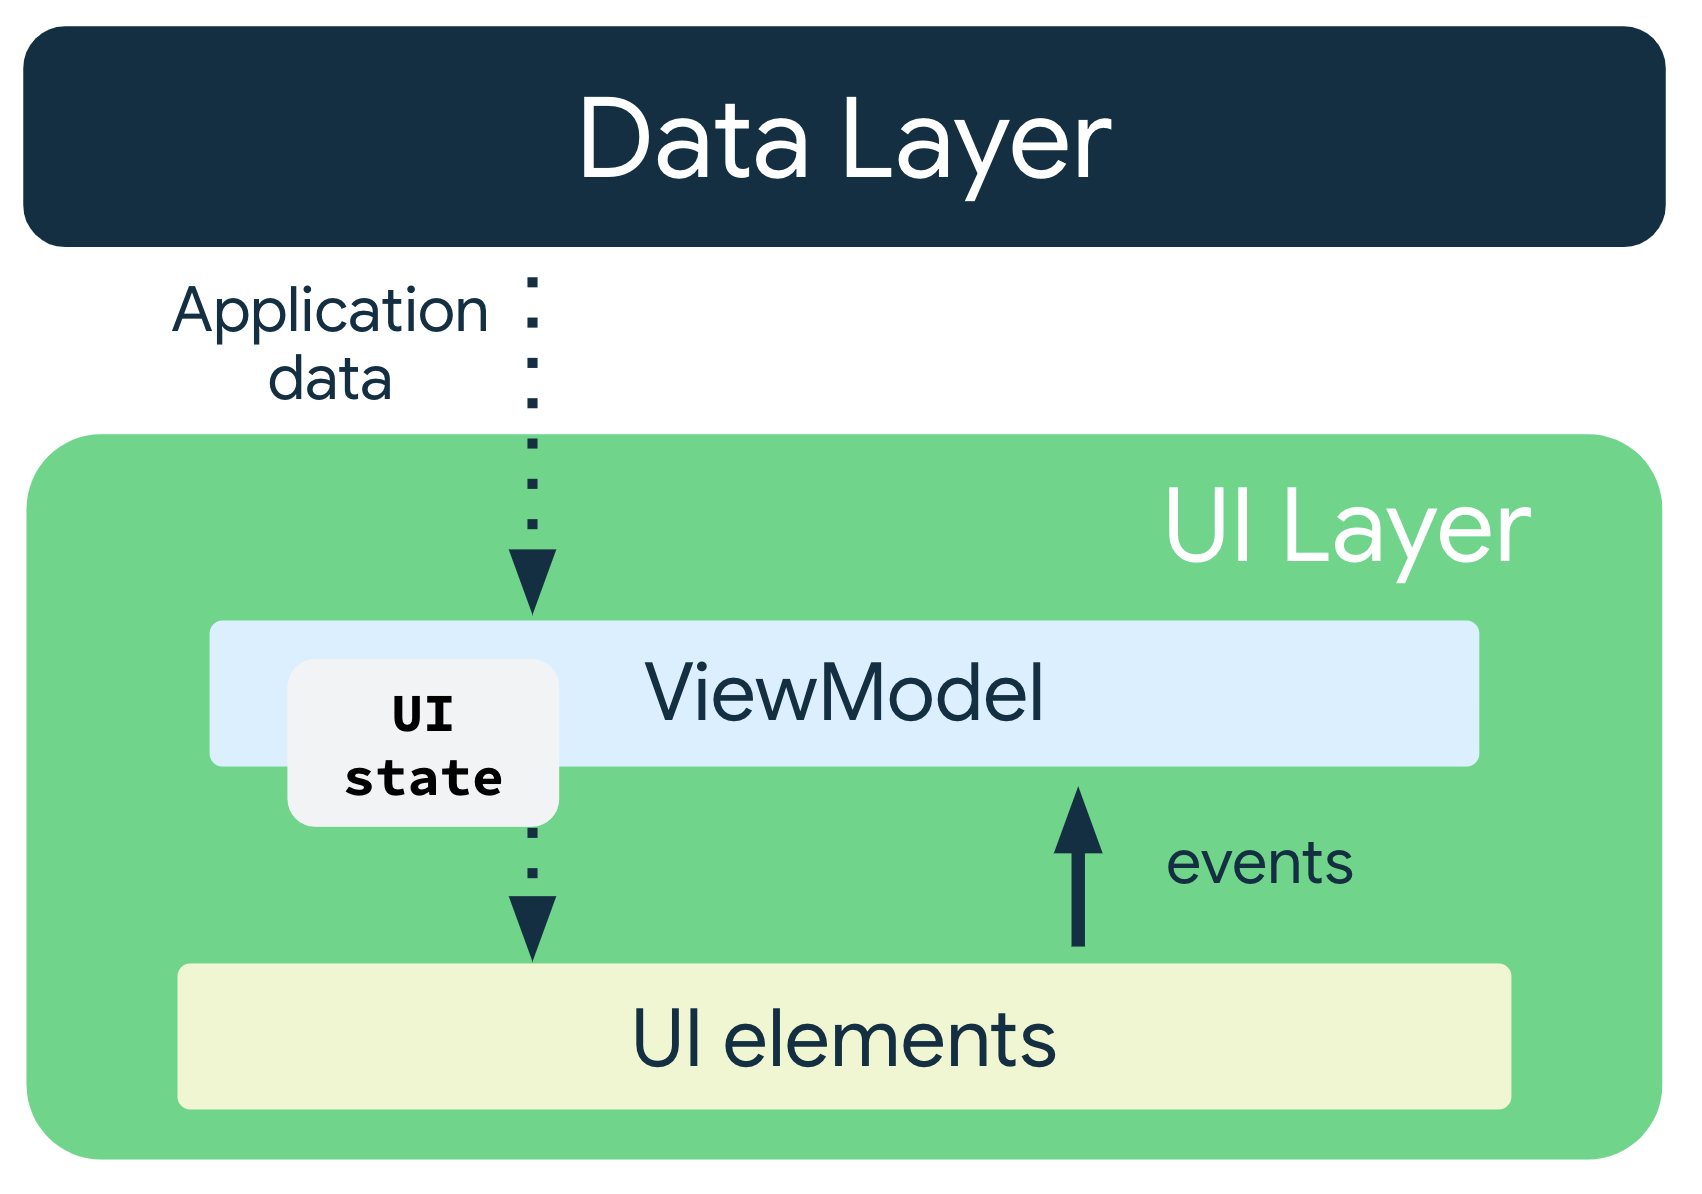
\includegraphics[width=\textwidth]{graphics/android_udf}
        \caption{Diagram of \gls{udf} in app architecture \cite{android_ui_layer}}
        \label{fig:android_udf}
    \end{subfigure}
    \hfill
    \begin{subfigure}[b]{0.4\textwidth}
        \centering
        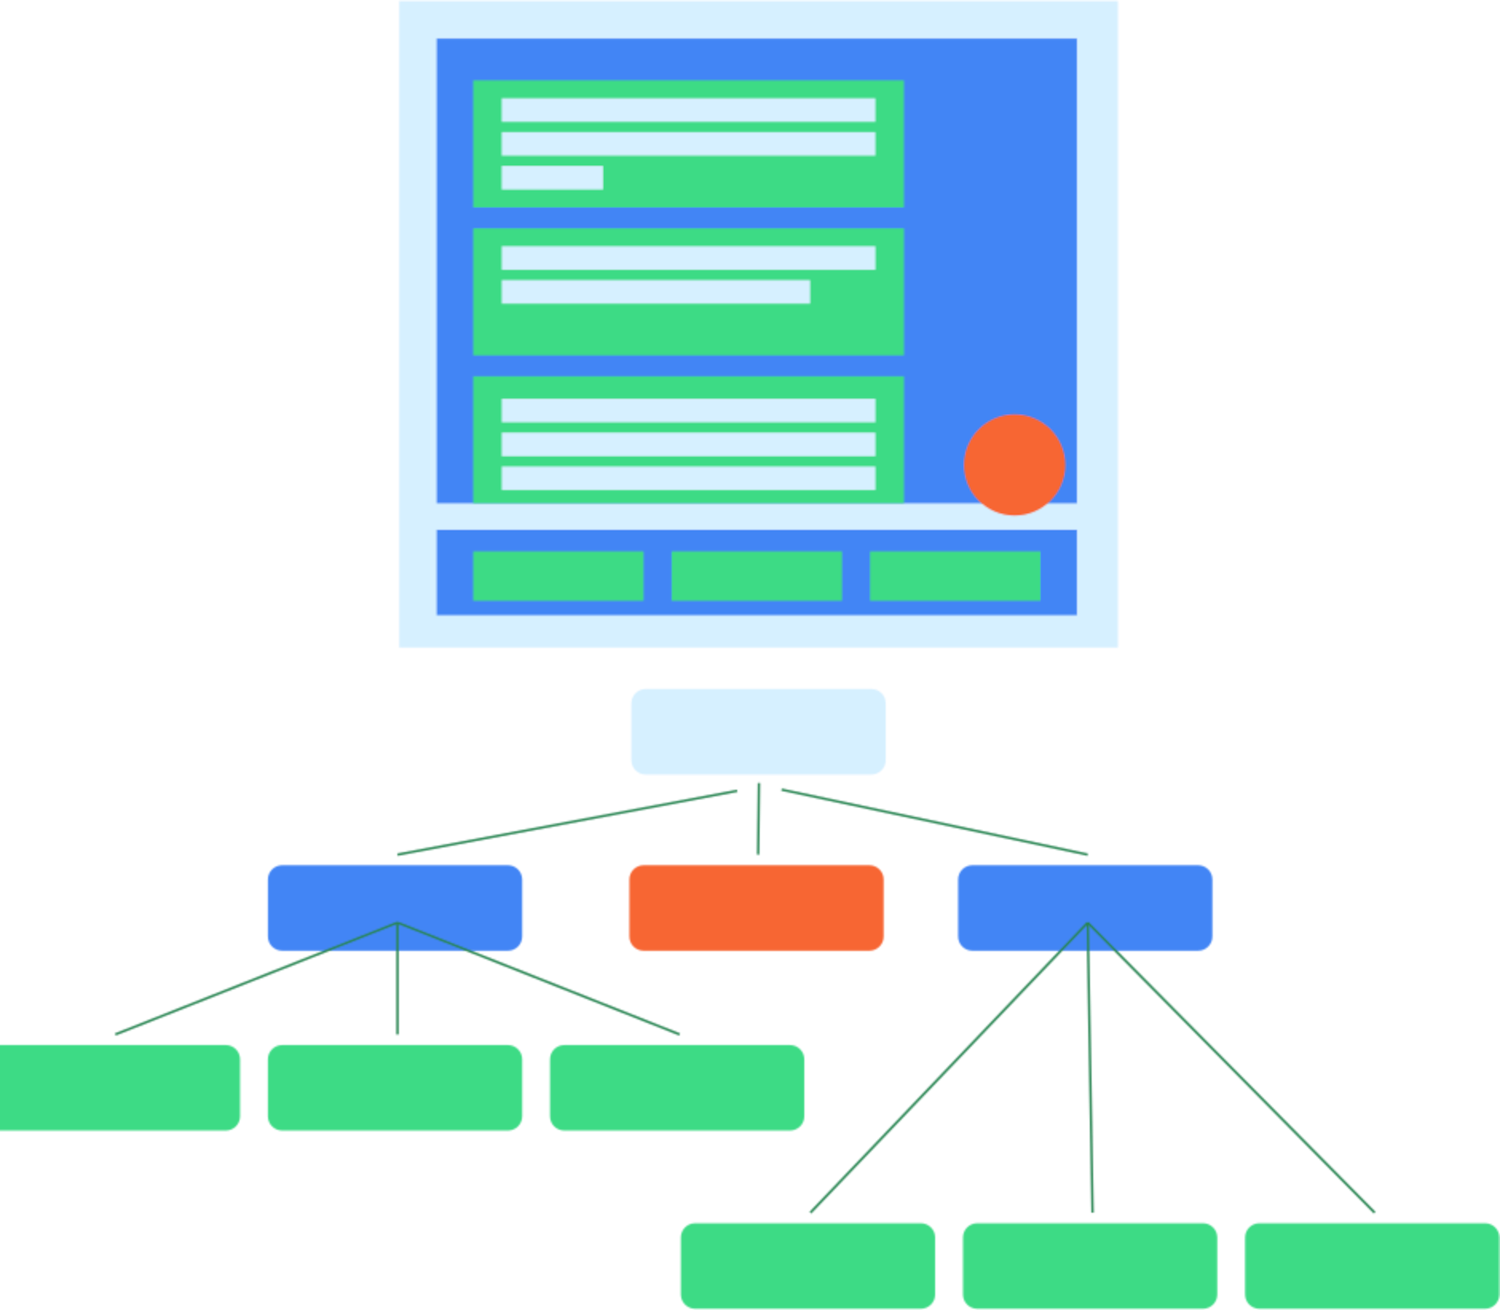
\includegraphics[width=\textwidth]{graphics/android_semantics-ui-tree}
        \caption{Schema of how the semantics tree is related to the \gls{ui} hierarchy \cite{android_semantics_compose}}
        \label{fig:android_semantics_ui_tree}
    \end{subfigure}
    \caption{Structure of the Android \gls{ui}}
    \label{fig:android_tree}
\end{figure}
%https://developer.android.com/guide/topics/ui/how-android-draws \cite{android_draw_views}
%https://developer.android.com/jetpack/compose/mental-model \cite{android_jetpack_compose}

\subsection{Data tree structure}
\label{subsec:data-tree-structure}

The \gls{ui} elements (i.e.\ the composition) themselves are hierarchically structured in a tree.
This allows the renderer to calculate relative distances, floatings and skip processing hidden or overlapped elements.

With the Android Layout Inspector (figure~\ref{fig:android_layout_inspector}) a view hierarchy tree can be visually inspected while displaying its position and layout on the Android screen.
Also, the layout attributes can be validated.
This tool allows to debug complex \gls{ui}s especially when using nested components and display them in a simplistic way.
Note that this tool is only available if one has access to the app's source code.

\begin{figure}[htbp!]
    \centering
    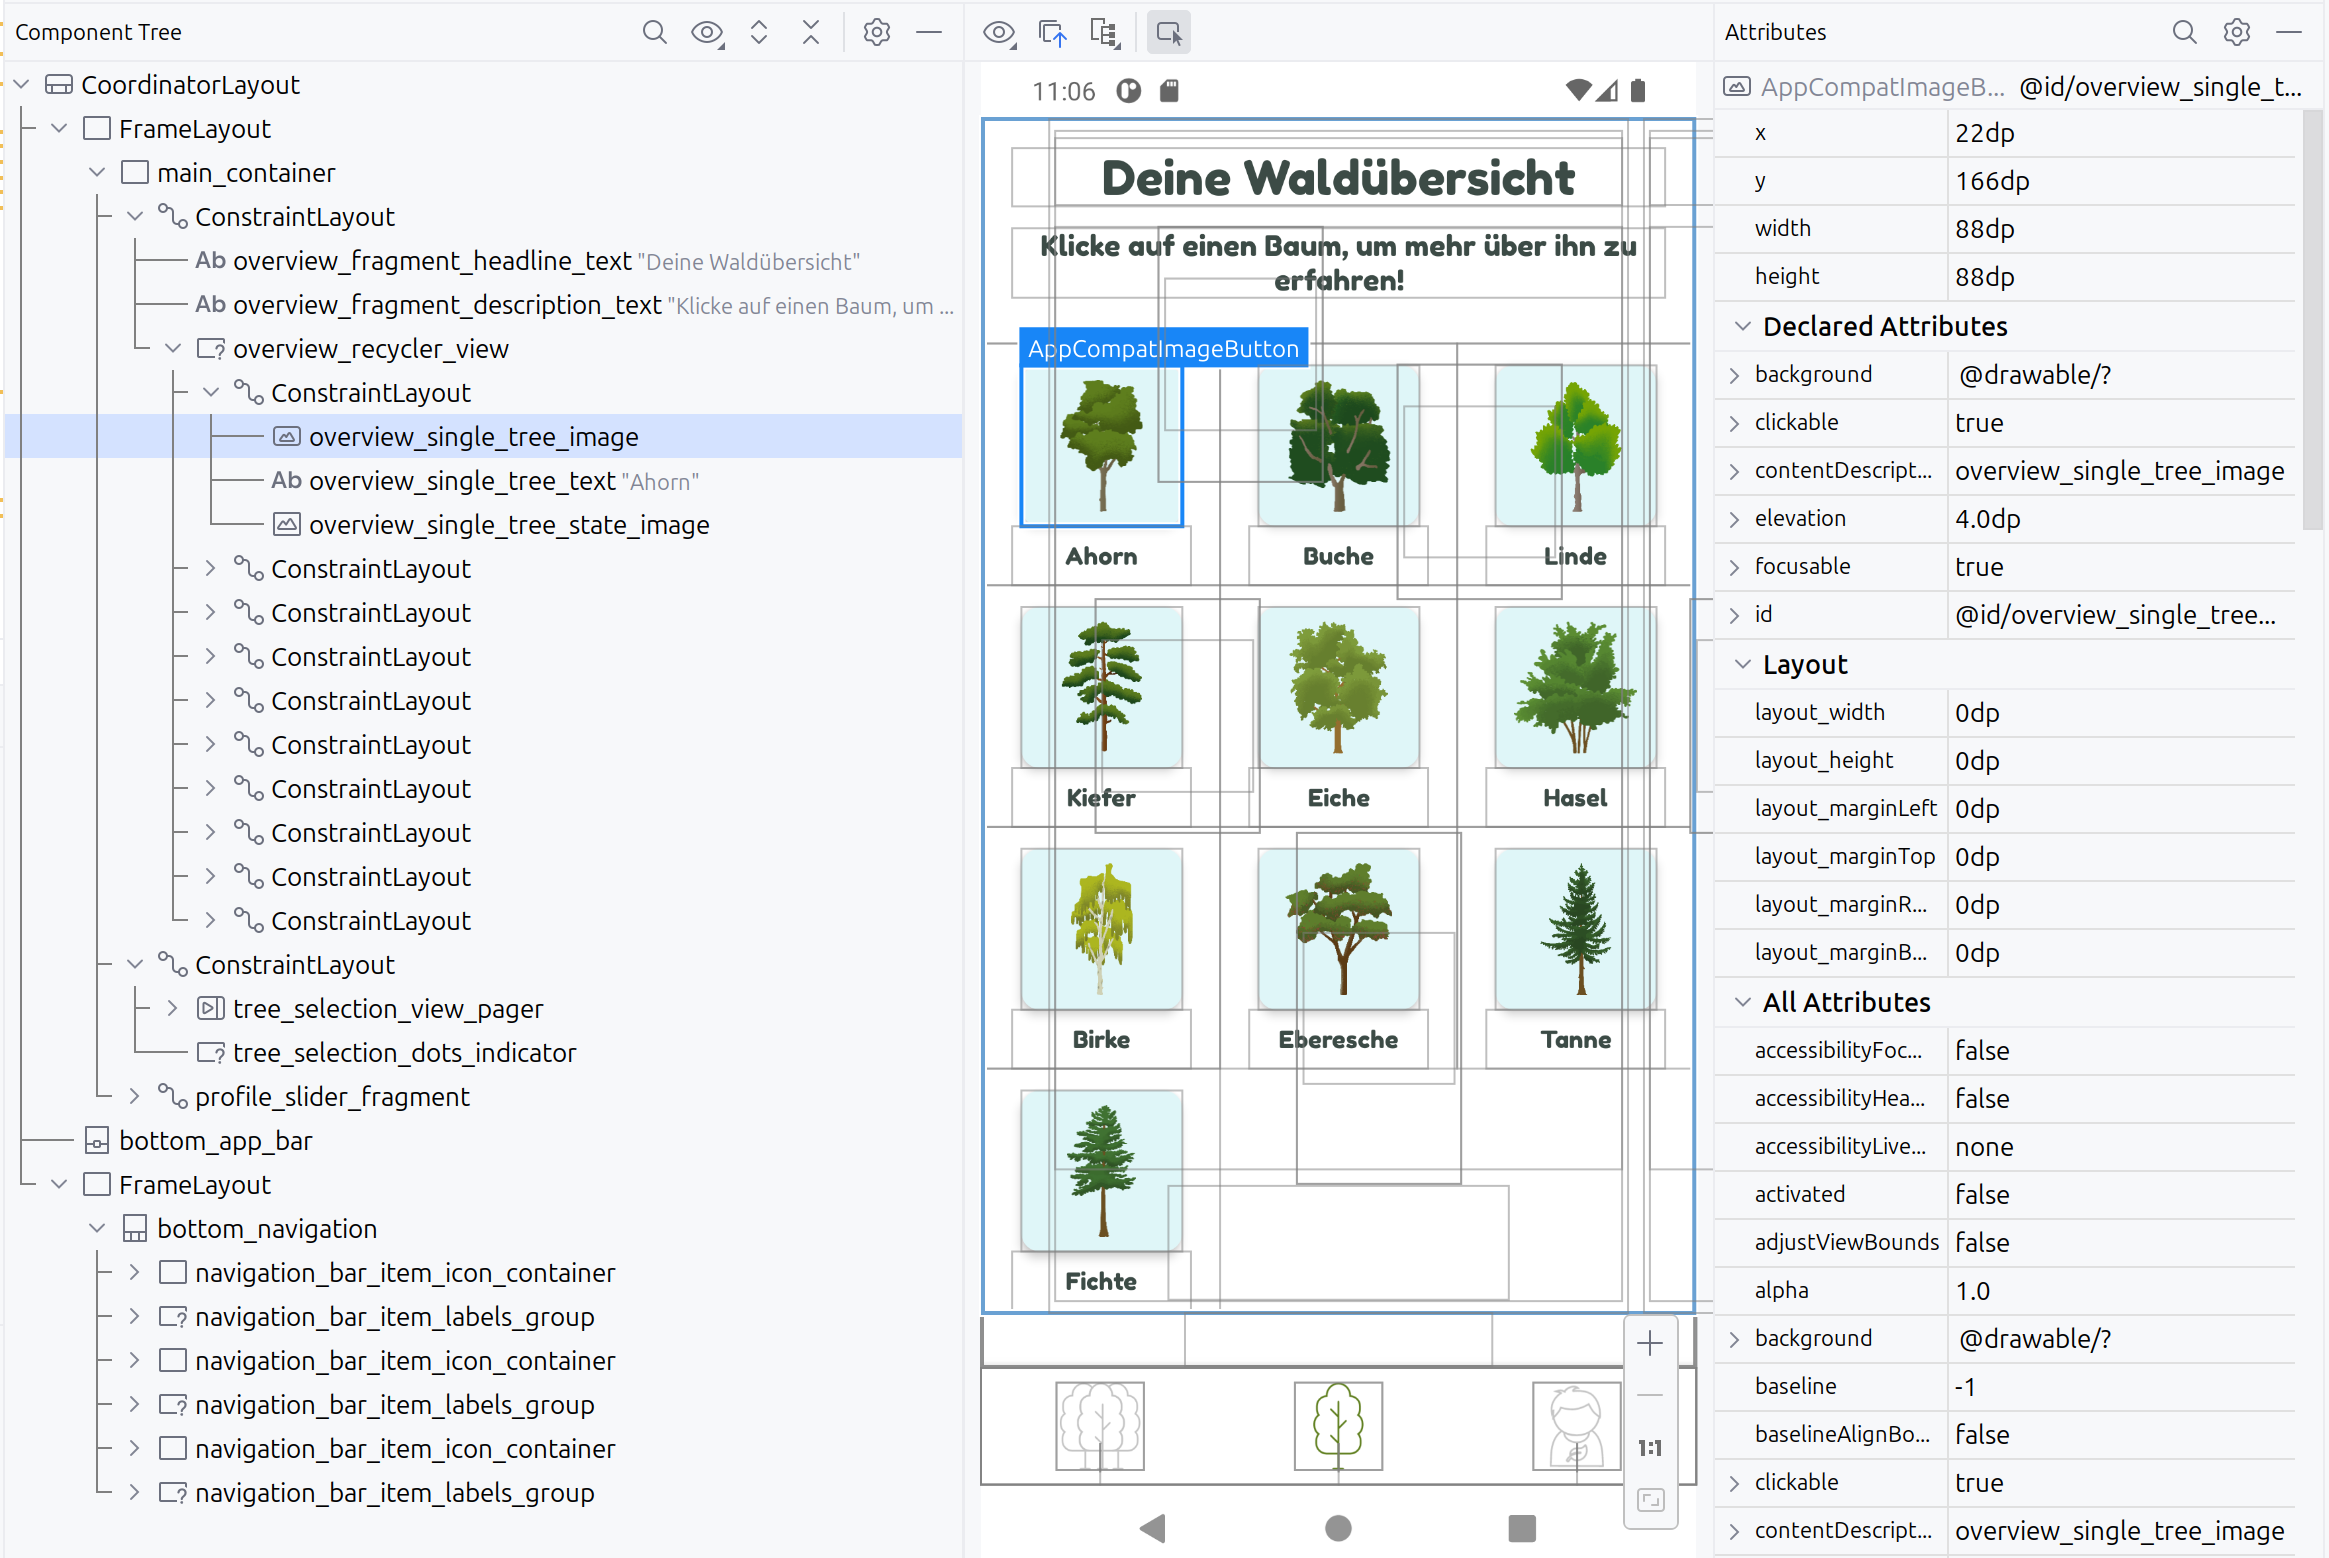
\includegraphics[width=\textwidth]{graphics/android_layout_inspector}
    \caption{The Android Layout Inspector tool using the example of \quotes{App ins Grüne}~\cite{mimuc_app_ins_gruene} by the Media Informatics Group of the LMU in Munich.}
    \label{fig:android_layout_inspector}
\end{figure}

\subsection{Android Accessibility Service}
\label{subsec:android-accessibility-service}

If an app is running in production on a users device, meaning that the app is compiled and publicly available, the ways of accessing the Android \gls{ui} tree are limited.
This behavior is of course wanted for safety and privacy reasons.
Nonetheless, if desired, a user can explicitly allow certain apps to gain access to the semantics tree of your Android \gls{os}.
This is especially useful for providing accessibility services for impaired users (like done with the TalkBack app).
Or -- as in our case -- the setting can be used to enable services which collect data for user studies or scientific experiments.

This semantics tree is deviated from the existing \gls{ui} tree.
It can be fed via special semantic properties while composing the \gls{ui}, e.g.\ by specifying the \code{contentDescription} property of an icon \cite{android_semantics_compose}.
Providing semantics is not limited to native platforms as shown by Flutter~\cite{flutter_semantics} and React Native~\cite{react_native_accessibility}.
In figure~\ref{fig:android_semantics_ui_tree} a schema is presented, which shows how the elements of the semantics tree are spanned compared to the components on the \gls{ui} layer.

%https://github.com/android/codelab-android-accessibility
To take advantage of the semantics tree, a custom accessibility service can be built, which can run in the background.
This service tracks all UI changes and has access to the current view hierarchy of the screen, which also inherits the semantic tree.
By altering the code of the \ti{AccessibilityNodeInfoDumper} one can extract the view hierarchy to a locale or remote database~\cite{android_accessibility_node_info_dumper}.
In the code section \ref{android_accessibility_node} a small fraction of a view hierarchy is shown.
It contains nested nodes with various attributes which represent the components of the combined \gls{ui} and semantics hierarchy.

%Semantics tree:
%https://api.flutter.dev/flutter/widgets/Semantics-class.html
%https://developer.android.com/jetpack/compose/semantics
%https://android.googlesource.com/platform/frameworks/testing/+/jb-dev/uiautomator/library/src/com/android/uiautomator/core/AccessibilityNodeInfoDumper.java \cite{android_accessibility_node_info_dumper}
%https://github.com/Gustl22/android-accessibility/blob/c158808533d6fc017455184a7317555d3e6946f6/GlobalActionBarService/app/src/main/java/com/example/android/globalactionbarservice/uiautomator/AccessibilityNodeInfoDumper.java

%Mean 18 actionable elements, with Std=12. \cite{zhou2021large}

\lstinputlisting[language=XML,label=android_accessibility_node,caption={Android Accessibility Node in XML.},float]{code/android_accessibility_node.xml}

\section{Machine Learning}
\label{sec:machine-learning}

\gls{ml}, a term spread by Arthur Lee Samuel, is a method of data analysis, more precisely a scientific approach to form statistical models without the need to explicitly program it~\cite{mahesh2020machine}.
It uses algorithms to iteratively learn how data is structured.
In contrast to statistical inference or manually crafted statistical models respectively, \gls{ml} can solve tasks by automation of model building.
Its advantages lie in finding hidden relations and patterns from the context, without having any or only a small pre knowledge of the data, thus it is a strong tool for generalization or abstraction of large datasets, also known as \gls{gl-bigdata}.
\gls{ml} can be applied to the following fields among others: email and spam filtering, fraud detection, cybersecurity, web search engines, recommender systems (like known from Netflix or Amazon), advertising, translators and text generation, pattern and image recognition.
The data driven approach also comes with some drawbacks: the outcome heavily depends on the provided data.
It can include biases and therefore may acquire forms of discrimination or unfair treatment.
Nonetheless \gls{ml} has a lot of potential to uncover hidden connections in large datasets.


\todo{explain Tensors, Datasets}
%https://stackoverflow.com/a/48599383/5164462

\subsection{Preprocessing}

Preprocessing describes the step after one acquired their data, but before training the \gls{ml} model.
This step is not to be underestimated.
A \gls{ml} model can perform significantly better when certain preprocessing steps are applied \cite{alam2019impact}.

To be able to preprocess, we have to know with what kind of data we handle with.
Data entries can occur in different forms, but we can break them down in three main types:
\begin{itemize}
    \item \tb{Categorical values}: a value is always assigned to a class with a fixed pool of predetermined classes.
          E.g.\ letters, words, brands, animals, chemical elements
    \item \tb{Continuous values}: the value can be fractional and may lies in between a lower and an upper bound.
          E.g.\ temperature, velocity, geographic position
    \item \tb{Integer values}: the value is a whole number and may also lie in between a lower and an upper bound.
          E.g.\ revolutions per minute, product number, annual sales
\end{itemize}

For discrete and continuous values, we have a wide variety of options for preparing them in order to be subsequently processed by a \gls{ml} model \cite{duong2021}.


\subsubsection{Feature selection}

Feature selection is a crucial step to successfully develop a model with the desired results.
It can improve learning performance, thus reduces time, increases computational efficiency, decreases memory storage, and helps build better generalization models \cite{li2017feature}.
Also, it may be a valid approach to get around missing data and can help structure the data by removing unnecessary clutter.

%https://dl-acm-org.emedien.ub.uni-muenchen.de/doi/pdf/10.1145/3136625
On the technical sight, feature selection can be differentiated for two goals: supervised and unsupervised learning~\cite{li2017feature}.
However, principles from the supervised feature selection can be applied in the unsupervised domain, resulting in a semi-supervised filter selection.
For classifiers and regression problems (unsupervised) following methods can be applied.
Multiple features can be compared by calculating their correlation.
If one feature is uncorrelated to all other features, this may be an indicator that this feature can be dropped, as it may doesn't contribute to the resulting model (\ti{filter method}).
However, this can only be stated for linear correlations, thus it may contribute to the result in an unpredicted way.
Also, if two features correlate too much to each other, one feature may is redundant and can be dropped.
A good approach is also to reduce the dimensionality of the input data, e.g.\ by replacing \ref{one-hot} encoded features of the same domain with embeddings (\ti{embedded method}).
This is also called \ti{feature extraction}.
Feature extraction can also be used in unsupervised feature selection.
Clustering is a common approach to reduce the number of input dimensions by gaining insights of which classes can be merged and which need to stay.
A more computational but promising solution is to filter the features by optimizing the model result, also called a \ti{wrapper method}.
By gradually removing and adding features and calculating the models performance, one can determine which inputs are important and which may only steal computing time.

\todo{formulate or remove}
semantic or legal feature selection
Such as Filtering privacy invasive details
Remove sensitive data
%https://news.mit.edu/2023/new-way-look-data-privacy-0714

Parameterizing the vectorization process
a) Vector length
b) Weighting of features
c) Manipulating individual parameters of model

\subsubsection{Missing data}
Some data entries may are missing.
Therefore, you have two approaches to get around these missing values.
One can drop these values by removing the column or row.
This is only recommended if you are not relying on this data entry, or this the whole feature is not expected to be important enough to bring any value to the model's performance.
Further you can fill the data with a default value like zero or calculate a reasonable value from the surrounding data entries by taking their \quotes{mean, median, or interpolation}~\cite{duong2021}.
The second approach can only be applied to numerical data.

\subsubsection{Normalization and Standardization}

This is only applicable for numerical data.
Many \gls{ml} models work better or exclusively with normalized data.
This means that the values have to be in a certain range, most commonly are from \tb{0} to \tb{1} or from \tb{-1} to \tb{1}.
This can be achieved by dividing all values with the difference of the minimum and maximum value and shift the output accordingly \cite{duong2021}.

% X new = (X — X min)/ (X max — X min)

Sometimes this is not enough, e.g.\ if having a few extreme values, and an approach is desired which better reflects the average data.
Here the standardization, also called z-score normalization, comes into play.
This method scales the values so that the mean value is placed at \tb{0} and the standard deviation is placed at \tb{1}.
%https://medium.com/analytics-vidhya/what-are-data-standardization-and-data-normalization-f880dd9e79b6
\subsubsection{Padding}


\subsubsection{Categorical Variables}

\todo{categorical}
According to \cite{alam2019impact} these steps can be removal of emoticons, elimination of stopwords and stemming for text based models.

ordinal categories belong to the \tb{Integer values} as they

Category Embedding before LSTM
% https://stackoverflow.com/questions/47217151/keras-lstm-with-embedding-layer-before-lstm-layer
% https://stackoverflow.com/questions/52627739/how-to-merge-numerical-and-embedding-sequential-models-to-treat-categories-in-rn/52629902#comment136040845_52629902


- Embedding layer
Embedding dimension is about the actual voc\_size, but not too large.
Dimension near the actual average length of features (?)

\subsection{Supervised vs Unsupervised vs Semisupervised}

\subsubsection{Supervised Learning}
Supervised: Classification and regression
Uses \tb{labeled} examples: Input and output is known

Learns by comparison of the output it is provided with the output the model \ti{predicts}.

Steps:
- Data acquisition
- Data cleaning / Preprocessing (Panadas)
- Split into Training Data, Validation data, and Test data (cannot adapt the model after using the test data)
- Train the model with the train data
- Evaluate the model with the test data, then can adapt the model by the developer
- Last deploy the model to production

\subsubsection{Unsupervised Learning}
Clustering
Reinforcement learning

self-supervised

\subsection{Under and Overfitting}
\label{subsec:under-and-overfitting}


\section{Artificial Neural Nets}
\label{sec:artificial-neural-nets}

- Uses biological neuron systems as paradigm to generate mathematical models
- can solve tasks by abstraction or generalization of data relations


Activation Functions
Cost function
Gradient
- Regression: Continous Values
- Classification: Multiple class
- One Class

\subsection{Classes of Neural Nets}
\label{subsec:classes-of-neural-nets}

\subsubsection{Deep Neural Nets}

Neural Net with more than one layer
- Dense Layer

\subsubsection{Convolutional Neural Nets}
\subsubsection{Recurrent Neural Networks and LSTMs / GRU}
LSTM 4 dimensional
% https://stackoverflow.com/questions/54743549/is-it-possible-to-making-lstm-model-with-4-dimension-shape-of-data

Limitations to only 3 dimensions, needs flattening

Sample dimension (X -> y)
Time (Step) Dimension
Feature Dimension
Data, Quantity dimension, such as Image dimensions, or multiple nodes

TimeDistributedLayer
% https://stackoverflow.com/a/61588937/5164462
% https://stackoverflow.com/questions/53107126/what-are-the-uses-of-timedistributed-wrapper-for-lstm-or-any-other-layers

\subsubsection{Autoencoders}
\label{subsubsec:autoencoder}

Encoder, Decoder

\subsection{Tensorflow and Keras}
Layers
FlattenLayer

Positive Integer to Dense Vectors of fixed size

\section{Evaluation and Metrics}
\subsection{Mean Squared Error}
\subsection{F1 Score}
